% Template for ICIP-2017 paper; to be used with:
%          spconf.sty  - ICASSP/ICIP LaTeX style file, and
%          IEEEbib.bst - IEEE bibliography style file.
% --------------------------------------------------------------------------
\documentclass{article}
\usepackage{spconf,amsmath,graphicx,Geoff}

% Example definitions.
% --------------------
%\def\x{{\mathbf x}}
%\def\L{{\cal L}}

% Title.
% ------
\title{A Graph-Based Approach for Feature Extraction and Segmentation of Multimodal Images}
%
% Single address.
% ---------------
\name{Geoffrey Iyer$^1$, Jocelyn Chanussot$^{1,2,3}$, Andrea L. Bertozzi$^{1}$}
\address{1. University of California, Los Angeles \\2. Univ. Grenoble Alpes, CNRS, GIPSA-lab, F-38000 Grenoble, France  \\3. Faculty of Electrical and Computer Engineering, University of Iceland, 101 Reykjavik, Iceland }
%
% For example:
% ------------
%
% Two addresses (uncomment and modify for two-address case).
% ----------------------------------------------------------
% \twoauthors
%   {A. Author-one, B. Author-two\sthanks{Thanks to XYZ agency for funding.}}
% 	{School A-B\\
% 	Department A-B\\
% 	Address A-B}
%   {C. Author-three, D. Author-four\sthanks{The fourth author performed the work
% 	while at ...}}
% 	{School C-D\\
% 	Department C-D\\
% 	Address C-D}


% TODO List:
% 1) Abstract
% 2) Keywords
% 3) Add to intro. Compare better with cca
% 4) Decide if I want two sets or many. Make the corresponding changes.
% 6) qualitative evaluation of results
% 7) A conclusion
% 8) Big literature search to get more references.
\begin{document}
% 
\maketitle
%
\begin{abstract}
  In the past few years, graph-based methods have proven to be a useful tool in
  a wide variety of energy minimization problems \cite{1262177}.  In this paper,
  we propose a graph-based algorithm for feature extraction and segmentation of
  multimodal images. By defining a notion of similarity that integrates
  information from each modality, we merge the different sources at the data
  level. The graph Laplacian then allows us to perform feature extraction and
  segmentation on the fused dataset. We apply this method in a practical
  example, namely the segmentation of optical and lidar images. The results
  obtained confirm the potential of the proposed method.
  % By constructing a graph, we integrate the different information sources at
  % the data level, producing a feature space that fuses the modalities into one
  % coherent structure.
  % By creating a notion of distance in multimodal sets that preserves the
  % independent information in each modality, and integrating the different sets
  % at the data level, we achieve more accurate segresults than
\end{abstract}

\begin{keywords}
  Image segmentation, multimodal image, data fusion, graph Laplacian,
  Nystr\"{o}m extension, graph cut minimization
\end{keywords}

\section{Introduction}
\label{sec:intro}

% This is supposed to answer the following questions: what do we want to adress
% (multimodal image processing) ?  what do people do in the litterature ?  what
% are potetial shortcomings ?  consequence-> our proposal (brief) announce the
% outline of the paper

With the increasing availability of data we often come upon multiple datasets,
derived from different sensors, that describe the same object or phenomenon. We
call the sensors \emph{modalities}, and because each modality represents some
new degrees of freedom, it is generally desirable to use more modalities rather
than fewer. For example, in the area of speech recognition, researchers have
found that integrating the audio data with a video of the speaker results in a
much more accurate classification \cite{Potamianos03,
  sedighin:hal-01400542}. Similarly, in medicine, the authors of \cite{Lei12}
and \cite{Samadi2016} fuse the results of two different types of brain imaging
to create a final image with better resolution than either of the
originals. However, correctly processing a multimodal dataset is not a simple
task \cite{lahat:hal-01062366}. Even the naive method of analyzing each modality
separately still requires clever thinking when combining the results, and this
is rarely the optimal way to handle the data. In this paper, we will instead
perform feature extraction on the full dataset, considering each modality
simultaneously. After creating a feature space, we can then use any standard
segmentation method to create a classification result.

Here we consider the case where each dataset contains the same number of
elements, and these elements are co-registered (so the $i$-th point in one set
corresponds to the $i$-th point in another). This often occurs in image
processing problems, where the sets may be images of the same scene obtained
from different sensors (as is the case in our experimental data), or taken at
different times. This problem has also been addressed in \cite{Tochon2015,
  Ali08}, although with different methods.

For notation, we label the sets, $X^1,X^2,\ldots,X^k$, with dimensions
$d_1,d_2,\ldots,d_k$, $\abs{X^j}=n$, and we let
\begin{align}X = (X^1,X^2,\ldots,X^k)\subset \R^{n\times (d_1+\cdots+d_k)}\end{align} be the
concatenated dataset. Our method extracts features from the dataset by finding
eigenvectors of the graph Laplacian, then uses standard data-segmentation
algorithms on these features to obtain a final classification.  In section
\ref{sec:method} we give the general theory behind our method, and in
\ref{sec:experiment} we show the results of the method applied to an
optical/LIDAR dataset.

% ----------------------------------------- Introduction from 1-15-2017,
% outdated now ----------------------------------------- With the increasing
% availibility of data we often come upon multiple datasets, derived from
% different sources, that describe the same object or phenomenon. These are
% called \emph{multimodal datasets}, and a proper treatment of such sets
% requires more than analyzing each set individually. One common practice is to
% define maps from each set into a common latent space, then perform any
% analysis on this common data. (TODO: talk about canonical correlation
% analysis, and maybe look up parallel factor analysis. I found this in
% \cite{Lahat15}.) These methods aim to find and correlate the redundant
% information between the different sets, however they struggle to identify any
% information that is exclusive to one dataset. Here we present a graph-based
% approach that aims to use the unique information found in each dataset to give
% a more detailed explanation of the source object.

% In this paper we consider the case where each dataset contains the same number
% of elements, and these elements are co-registered (so the $i$-th point in one
% set corresponds to the $i$-th point in another). This situation is often found
% in image processing, where the sets may be images obtained from different
% sources (as is the case in our experimental data), or taken at a different
% time. Call the sets, $X^1,X^2,\ldots,X^m$, with dimensions
% $d_1,d_2,\ldots,d_m$. Let
% $X = (X^1,X^2,\ldots,X^m)\subset \R^{n\times (d_1+\cdots+d_m)}$ be the
% concatenated dataset. Our method creates a latent space $Y$, along with a map
% $X\to Y$. We then use $k$-means to segment the data in $Y$ apply this
% segmentation to $X$. In section \ref{sec:method} we give the general theory
% behind our method, and in \ref{sec:experiment} we show the results of the
% method applied to an Optical/LIDAR dataset.

% ----------------------------------------- A random paragraph from 12/2016. Not
% sure why we have this -----------------------------------------
%%% In this paper we address the question of segmentation of multimodal
%%% datasets. We provide an unsupervised method for data classification Blah
%%% blah blah blah. Two datasets, $X^s$, $X^t$, that describe the same
%%% object. Our goal is to somehow combine the sets to form one set $Y$ that
%%% blah blah. In the general scenario, $X^s$ and $X^t$ will often contain
%%% redundant information. Previous methods attempt to correlate the redundant
%%% parts of the two sets, but this often results in a overall loss of
%%% information, as the data unique to the individual sets isn't properly
%%% considered. In this paper we aim to emphasize the nonredundant data in our
%%% creation of $Y$.  Maybe we set up some notation here.

\section{The Method}
\label{sec:method}

\subsection{Graph Laplacian} \label{sec:GraphLaplacian} We approach this problem
via graph-based methods. A more detailed survey of the theory can be found in
\cite{vonLuxburg07}. Here we state only the results necessary to implement our
algorithm.

\subsubsection{The Graph Min-Cut Problem} \label{sec:GraphMinCut} We represent
our dataset $X$ using an undirected graph $G = (V,E)$. The nodes $v_i\in V$ of
the graph correspond to elements of $X$, and we give each edge $e_{ij}$ a
\emph{weight} $w_{ij}\geq 0$ representing the similarity between nodes
$v_i, v_j$, where large weights correspond to similar nodes, and small weights
to dissimilar nodes. This gives rise to a \emph{similarity matrix} (also called
the \emph{weight matrix})
\begin{align}W = \left(w_{ij}\right)_{i,j=1}^n.\end{align} Since $G$ is undirected, we require that
$w_{ij} = w_{ji}$, which implies that $W$ is a symmetric matrix. There are many
different notions of ``similarity'' in the literature, and each has its own
merits. In many applications, one defines
\begin{align}w_{ij} = -\text{exp}\left(\norm{v_i -v_j} / \sigma \right),\end{align} where $\sigma$
is a scaling parameter. In this work we adapt this definition to apply to our
multimodal dataset, as is explained in \ref{sec:Weights}.

Once the weight matrix has been defined, the data clustering problem can be
rephrased as a graph-cut-minimization problem of the similarity matrix
$W$. Given a partition of $V$ into subsets $A_1,A_2,\ldots,A_m$, we define the
\emph{ratio graph-cut}
\begin{align}
  \text{RatioCut}(A_1,\ldots,A_m) = \frac{1}{2}\sum_{i=1}^m
  \frac{W(A_i,A_i^c)}{\abs{A_i}}.
\end{align}
Where
\[W(A,B) = \sum_{i\in A, j\in B}w_{ij},\] and the $\frac{1}{2}$ is added to
account for double-counting each edge.  Heuristically, minimizing the ratio cut
serves to minimize the connection between distinct $A_i, A_j$, while still
ensuring that each set is of a reasonable size. Without the $\abs{A_i}$ term,
the optimal solution often contains one large set and $m-1$ small sets.

Solving the graph min-cut problem is equivalent to finding $m$ indicator vectors
$f_1,\ldots,f_m \in \R^n$ such that
\[f_{m,j} = \begin{cases} 1 & \text{ if } x_j \in A_m \\ 0 & \text{ else}
  \end{cases}.\] It has been shown in \cite{Goldschmidt94} that explicitly
solving this problem is an $O(\abs{V}^{m^2})$ process. As this is infeasible in
most cases, we instead introduce the graph Laplacian along with an approximation
of the minimization problem.

\subsubsection{Graph Laplacian} \label{subsec:GraphLaplacian} After forming the
weight matrix $W$, we define the graph Laplacian. For each node $v_i\in V$,
define the \emph{degree} of the node
\begin{align}d_i = \sum_j w_{ij}.\end{align} Intuitively, the degree represents the strength of a
node. Let $D$ be the diagonal matrix with $d_i$ as the $i$-th diagonal entry. We
then define the \emph{graph Laplacian}
\begin{align}
  L = D - W.
\end{align}
For a thorough explanation of the properties of the graph Laplacian, see
\cite{Mohar91}. In our work we will use that $L$ is symmetric and positive
definite, as well as the following fact (proven in \cite{vonLuxburg07}).
\begin{fact}
  For a given graph-cut $A_1,\ldots,A_m$, define the $f_1,\ldots,f_m$ as above,
  and have $h_j = f_j/\norm{f_j}$. Let $H$ be the $n\times m$ matrix whose
  columns are $h_j$. Then $H^T H = I$, and
  \begin{align}
    \text{RatioCut}(A_1,\ldots,A_m) = \text{Tr}\left(H^T L H\right).
  \end{align}
\end{fact}
As explained in \ref{sec:GraphMinCut}, we cannot solve this problem explicitly,
so instead we relax the problem to allow entries of $H$ to take on arbitrary
real values. That is, we find
\begin{align}
  \text{argmin}_{H\in \R^{n\times m}} \text{Tr}\left(H^T L H\right)\;\text{
  where }H^TH=I.
\end{align}
As $L$ is symmetric and $H$ is orthogonal, this problem is solved by choosing
$H$ to be the matrix containing the $m$ eigenvectors of $L$ corresponding to the
$m$ smallest eigenvalues. Using the eigenvectors $H$ we define a map
$X \to \R^m$. For each graph node $x_i\in X$ we get a vector
$y_i\in\mathbb{R}^m$ given by the $i$th row of $H$. These $y_i$ give the
solution to the relaxed min-cut problem, as such can be thought of as features
extracted from the original dataset $X$.

To obtain a solution to the original min-cut problem, we must then perform some
kind of classification on the $y_i$ to create the indicator vectors
$f_1,\ldots,f_m$ as described above. There is a large variety of such methods in
the literature (\cite{Hu2015,Merkurjev13} are some examples). In section
\ref{sec:experiment} we use $k$-means to segment the $y_i$, resulting in a
well-known algorithm called \emph{spectral clustering}. Although $k$-means is
unlikely to give an optimal classification, it is quite easy to implement, and
the final results are strong enough to give a proof-of-concept.

\subsection{Nystr\"{o}m Extension}\label{sec:Nystrom}
Calculating the full graph Laplacian is computationally intensive, as the matrix
contains $n^2$ entries. Instead we use Nystr\"{o}m's extension to find
approximate eigenvalues and eigenvectors with a heavily reduced computation
time. See \cite{Fowlkes04, Merkurjev13, Woodworth13} for a more complete
discussion of this method.

Let $X$ denote the set of nodes of the complete weighted graph. We choose a
subset $A\subset X$ of ``landmark nodes'', and have $B$ its complement. Up to a
permutation of nodes, we can write the weight matrix as
\begin{align}
  W = \begin{pmatrix} W_{AA} & W_{AB} \\ W_{BA} & W_{BB}
  \end{pmatrix},
\end{align}
where the matrix $W_{AB} = W_{BA}^T$ consists of weights between nodes in $A$
and nodes in $B$, $W_{AA}$ consists of weights between pairs of nodes in $A$,
and $W_{BB}$ consists of weights between pairs of nodes in $B$. Nystr\"{o}m's
extension approximates $W$ as
\begin{align}
  W \approx \begin{pmatrix} W_{AA} \\ W_{BA} \end{pmatrix}
  W_{AA}^{-1} \begin{pmatrix} W_{AA} & W_{AB}\end{pmatrix}.
\end{align}
where the error of approximation is determined by how well the rows of of
$W_{AB}$ span the rows of $W_{BB}$.
% CUT ON 2-6-17 ----- As $W$ is positive semidefinite, we can write it as a
% matrix transpose times itself $W = V^TV$. In \cite{Belongie2002}, the authors
% show that the Nystr\"{o}m extension estimates the unknown part of $V$
% (corresponding to $W_{BB}$) by orthogonally projecting it into the known part
% (corresponding to $W_{AB}$).  ------
This approximation is extremely useful, as we can use it to avoid calculating
$W_{BB}$ entirely. It is in fact possible to find $\abs{A}$ approximate
eigenvectors of $W$ using only the matrices $W_{AA},W_{AB}$. This results in a
significant reduction in computation time, as we compute and store matrices of
size at most $\abs{A}\times\abs{X}$, rather than $\abs{X}\times\abs{X}$.

In practice, the details of choosing $A$ will not significantly affect the final
performance of the algorithm. Although it is possible to choose specific
``landmark nodes'', in most applications (including ours) the elements of $A$
are selected at random from the full set $X$. Furthermore, the amount of
landmark nodes $m$ can be chosen to be quite small without noticeably affecting
performance. This makes Nystr\"{o}m's extension especially useful in application,
as very little work is required to tune the parameters.  In Section
\ref{sec:experiment} we use $m = n^{\frac{1}{4}}$, and choosing a larger set $A$
does not give a significant change in the error of approximation.

% NOTE: Could expand this section to further explain the approximation (it is an
% orthogonal projection of $W_{BB}$ onto $W_{AB}$), and how the eigenvectors are
% actually derived. This can all be found in \cite{Woodworth13}. If there is
% space I'll add it.

\subsection{Multimodal Edge Weights}\label{sec:Weights}

To calculate the weight matrix $W$, we first scale our sets $X^1, \ldots, X^k$
to make distances in each set comparable. Let
$X = (X^1, \ldots, X^k) \subset \R^{n\times (d_1+\cdots+d_k)}$ be the
concatenated dataset, and let $A\subset X$ be the collection of landmark nodes
as in \ref{sec:Nystrom}. For simplicity of notation, rearrange the entries of
$X$ so that $A = \{x_1,\ldots,x_m\}$.  So $\abs{A} = m$, and $m\ll n$. Then for
$\ell = 1,\ldots,k$ define the scaling factor
\begin{align}
  \lambda_\ell = \text{std}\left(\norm{x_i^\ell-x_j^\ell} ;\; 1\leq i\leq
  n,\; 1\leq j\leq m\right)
\end{align}
For a graph node $x\in X$, we define
\begin{align}
  \norm{x} = \max\left( \frac{\norm{x^1}}{\lambda_1},\cdots,
  \frac{\norm{x^k}}{\lambda_k}\right).
\end{align}
Then define the weight matrix $W$ (using the Nystr\"{o}m Extension), by
\begin{align}
  W = \begin{pmatrix} W_{AA} \\ W_{AB}
  \end{pmatrix} = (w_{ij})_{1\leq i \leq n, 1\leq j \leq m}
\end{align}
with $w_{ij} = \text{exp}\left(-\norm{x_i - x_j}\right).$

Note that the $\norm{\cdot}$ defined above is a norm on the concatenated dataset
$X$. We specifically choose to use the maximum of the individual measurements to
emphasize the unique information that each dataset brings. With this norm, two
data points $x_i,x_j$ are considered similar only when they are similar in each
dataset.

\section{Experiment}
\label{sec:experiment}

% Below is an example of how to insert images. Delete the ``\vspace'' line,
% uncomment the preceding line ``\centerline...'' and replace ``imageX.ps'' with
% a suitable PostScript file name.
% -------------------------------------------------------------------------
\begin{figure}[htb]
  \begin{minipage}[b]{0.48\linewidth}
    \centering
    \centerline{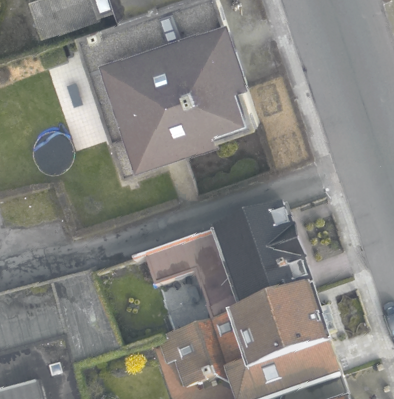
\includegraphics[width=3.8cm]{./Images/DFC2015/optical.png}}
    % \vspace{2.0cm}
    \centerline{(a) Optical data}\medskip
  \end{minipage}
%
  \begin{minipage}[b]{.48\linewidth}
    \centering
    \centerline{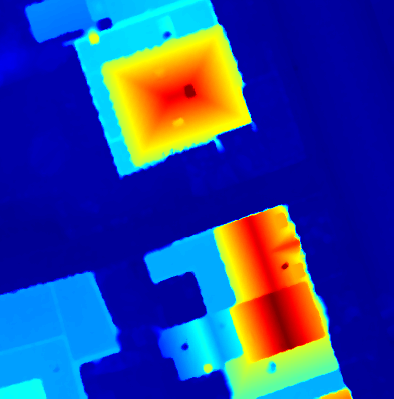
\includegraphics[width=3.8cm]{./Images/DFC2015/lidarColor.png}}
    % \vspace{1.5cm}
    \centerline{(b) Lidar data}\medskip
  \end{minipage}

  \begin{minipage}[b]{.48\linewidth}
    \centering
    \centerline{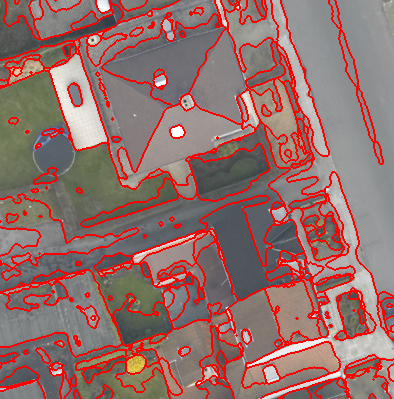
\includegraphics[width=3.8cm]{./Images/DFC2015/opticalOnly.png}}
    % \vspace{1.5cm
    \centerline{(c) Optical segmentation}\medskip
  \end{minipage}
%
  \begin{minipage}[b]{.48\linewidth}
    \centering
    \centerline{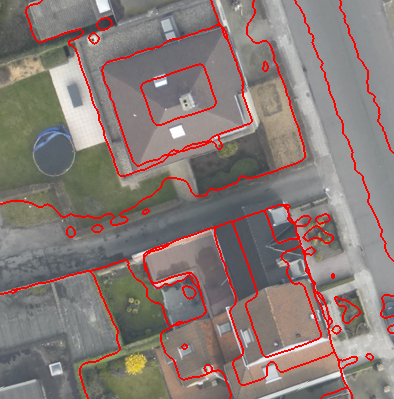
\includegraphics[width=3.8cm]{./Images/DFC2015/lidarOnly.png}}
    % \vspace{1.5cm}
    \centerline{(d) Lidar segmentation}\medskip
  \end{minipage}

  \begin{minipage}[b]{.48\linewidth}
    \label{fig:evec}
    \centering
    \centerline{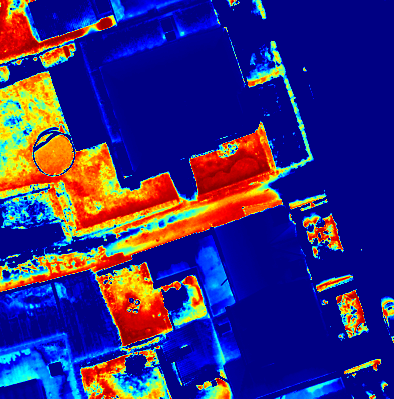
\includegraphics[width=3.8cm]{./Images/DFC2015/evecColor.png}}
    % \vspace{1.5cm
    \centerline{(e) Example eigenvector}\medskip
  \end{minipage}
%
  \begin{minipage}[b]{.48\linewidth}
    \centering
    \centerline{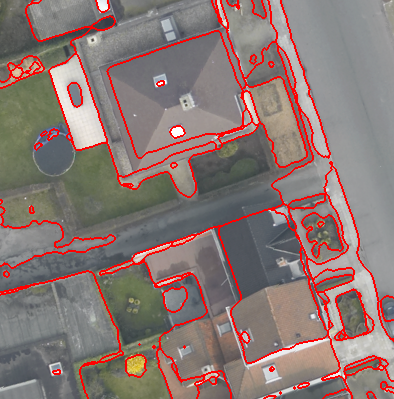
\includegraphics[width=3.8cm]{./Images/DFC2015/withBorders.png}}
    % \vspace{1.5cm}
    \centerline{(f) Our segmentation}\medskip
  \end{minipage}
  \caption{DFC Data Experimental Results.}
  \label{fig:experimentDFC}
\end{figure}

We test our algorithm on an optical/LIDAR dataset from the 2015 IEEE Data Fusion
Contest \cite{7536139}, shown in figure \ref{fig:experimentDFC}a,b. The data
consists of an RGB image and an elevation map of a residential neighborhood in
Belgium. We choose this particular scene because of the large amount of
non-redundancy between the two images. The lidar data is effective at
differentiating the roofs of the buildings from the adjacent streets, and the
optical data is useful for segmenting the many different objects at
ground-level. In figures \ref{fig:experimentDFC}c,d we show the results of
spectral clustering performed using each modality separately. The issues with
single-modality segmentation can be seen immediately, as both segmentations miss
out on key features of the data.

In figure \ref{fig:experimentDFC}e,f we show the results of our
method. \ref{fig:experimentDFC}e is one example eigenvector of the graph
Laplacian. As explained in \ref{subsec:GraphLaplacian}, this vector can be
considered one feature of our dataset, and approximates a segmentation of the
image into 2 groups. Notice how in this eigenvector the dark-grey street is
highlighted, while both the light-grey sidewalk (which is at the same elevation)
and the nearby roof (which is the same color) are dark. This shows at the
feature level that our algorithm is successfully using both the optical and the
lidar data when determining what pixels can be considered similar. The
difference shown in this example vector then causes the classification algorithm
to separate those regions in the final result \ref{fig:experimentDFC}f.  This
last figure was obtained using a total of 12 eigenvectors (not pictured here),
grouped into 5 classes.

\begin{figure}[htb]
  \begin{minipage}[b]{0.48\linewidth}
    \centering
    \centerline{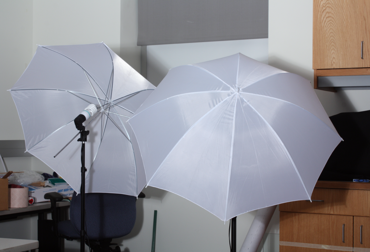
\includegraphics[width=3.8cm]{./Images/Umbrella/optical.png}}
    % \vspace{2.0cm}
    \centerline{(a) Optical data}\medskip
  \end{minipage}
%
  \begin{minipage}[b]{.48\linewidth}
    \label{fig:lidarData}
    \centering
    \centerline{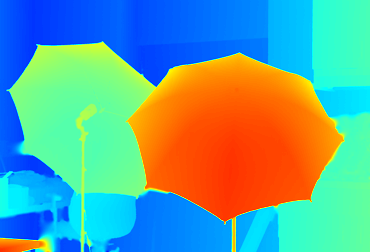
\includegraphics[width=3.8cm]{./Images/Umbrella/lidarColor.png}}
    % \vspace{1.5cm}
    \centerline{(b) Lidar data}\medskip
  \end{minipage}

  \begin{minipage}[b]{.48\linewidth}
    \label{fig:evec}
    \centering
    \centerline{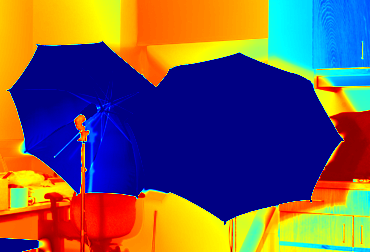
\includegraphics[width=3.8cm]{./Images/Umbrella/evecColor.png}}
    % \vspace{1.5cm
    \centerline{(c) Example eigenvector}\medskip
  \end{minipage}
%
  \begin{minipage}[b]{.48\linewidth}
    \centering
    \centerline{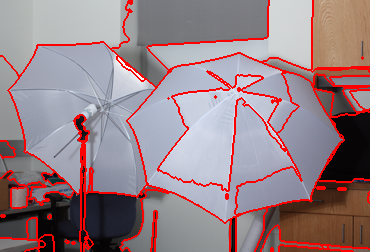
\includegraphics[width=3.8cm]{./Images/Umbrella/withBorders.png}}
    % \vspace{1.5cm}
    \centerline{(d) Our segmentation}\medskip
  \end{minipage}
  \caption{Umbrella Data Experimental Results}
  \label{fig:experimentUmbrella}
\end{figure}

In fig \ref{fig:experimentUmbrella} we show the results of our method applied to
another optical/lidar set (found in \cite{Scharstein14}). Similar to the DFC
set, the umbrella data serves as a good example because it cannot be easily
analyzed using one modality alone. The umbrellas and the background walls are
nearly the same shade of white, and can only be distinguised in the lidar
data. Meanwhile, the different pieces of the background all lie at nearly the
same depth, and can only be separated by color. As was the case with the DFC
data, the final classification \ref{fig:experimentUmbrella}d can be understood
by looking at the individual feature vectors. In \ref{fig:experimentUmbrella}c
we show the vector responsible for separating the umbrellas from the background
wall (using the lidar data), as well as from the black umbrella stands (using
the RGB data).

For a given segmentation of an image, computing the graph-cut error as described
in \ref{sec:GraphMinCut} is an $O(n^2)$ calculation, and requires the full
weight matrix $W$. To avoid this, we instead measure the error of segmentation
by how the data $X = (X^1,\ldots,X^k) \subset \R^{n\times (d_1+\cdots+d_k)}$
varies within each class. Explicitly, we use the metric:
% max method.
\begin{align}
  \text{Error} = \frac{1}{n}\sum_{\text{classes }\cC}\sum_{x\in \cC}\norm{x - \text{mean}\left(y\in \cC\right)}.
\end{align}
% Error here: my method is 0.4072 union method is 0.4377 2-norm method is 0.4140
% optical only is 0.8338 lidar only is 0.7504
%
% 
% std method. I think I did the math wrong here.
% \begin{align}
%   \text{Error} = \sum_{\text{classes }\cC}\text{std}\left(x \in \cC\right).
% \end{align}
% I don't have data for this method saved, which is probably dumb of me.
% 
Where the norm $\norm{\cdot}$ is the same as defined in \ref{sec:Weights}.

To test our method, we compare against a few other common methods. The results
are given in Table \ref{table:experimentQuantitative}. Unfortunately, due to
space limitations, we cannot display the visual comparisons between the
different algorithms. Instead we will briefly describe the methods used. The
2-norm on the concatenated set $X$ still minimizes a graph-cut, but uses a
slightly different norm to define the weight matrix
\begin{align}
  \norm{x} = \sqrt{\frac{\norm{x^1}^2}{\lambda_1} + \cdots +
  \frac{\norm{x^k}^2}{\lambda_k}},
\end{align}
where the scaling factors $\lambda_j$ are the same as in \ref{sec:Weights}.  The
intersection method computes the classification via spectral clustering on
$X^1, \ldots, X^k$ separately, then segments the data by intersecting the
individual classifications.

\begin{table}
  \centering
  \begin{tabular}{l l l}
    \textbf{Method} & \textbf{DFC error} & \textbf{Umbrella error}\\
    \textbf{Our method} & 0.40 & 0.31 \\
    Our method with 2-norm & 0.41 & 0.33 \\
    Intersection method & 0.43 & 0.51 \\
    Graph cut on optical only & 0.83 & 0.86 \\
    Graph cut on lidar only & 0.75 & 0.50 \\
    K-means on original data & 0.75 & 0.49 \\
  \end{tabular}
  \caption{Quantitative comparisons with other methods}
  \label{table:experimentQuantitative}
\end{table}

\section{Conclusions}
\label{sec:conclusions}

In conclusion, graph-based methods provide a straightforward and flexible method
of combining information from multiple datasets. By defining a weight map
$\R^{n\times\left(d_1+\cdots+d_k\right)}\to\R_{\geq 0}$ with some reasonable
norm-like properties, we can create the graph Laplacian of the data and extract
features in the form of eigenvectors. These features can then be used as part of
many different data-segmentation algorithms. For this paper, we use $k$-means on
the eigenvectors as a simple proof-of-concept. However this portion of our
method could easily be replaced with a more in-depth approach, such as a
Mumford-Shah model \cite{Hu2015}, or even a semi-supervised method such as
\cite{Merkurjev13}. Our next area of interest is the removal of the
co-registration assumption. In section \ref{sec:experiment} our two images are
of the same underlying scene, where pixels correspond exactly between images. We
could not, for example, process two images taken from different angles. Our goal
for the future is to remove this restriction and develop an algorithm that can
be applied more varied datasets.

This work was supported by NSF grant DMS-1118971, ONR grant N00014-16-1-2119,
NSF grant DMS-1417674, European Research Council (Grant no. 320684 - CHESS
project), and CNRS (Grant no. PICS-USA 263484)

% Cut on 2-05-17 ------------------------------------- One possible approach is
% through manifold alignment techniques, as in
% \cite{Yang13,Wang11,Yeh14}. However, using these methods will require a great
% deal of care, as the process of aligning manifolds often blurs out the unique
% information given by each modality, defeating the purpose of using a
% multimodal dataset.  -------------------------------------

% The main issue here would be to somehow correlate the redundant parts of the
% different modalities, while still preserving the unique information that each
% one brings.

% TODO: not till the very end though.
% \section{COPYRIGHT FORMS}
% \label{sec:copyright}

% You must include your fully completed, signed IEEE copyright release form when
% form when you submit your paper. We {\bf must} have this form before your
% paper can be published in the proceedings.

% References should be produced using the bibtex program from suitable BiBTeX
% files (here: strings, refs, manuals). The IEEEbib.bst bibliography style file
% from IEEE produces unsorted bibliography list.
% -------------------------------------------------------------------------

% % To start a new column (but not a new page) and help balance the last-page
% % column length use \vfill\pagebreak.
% % -------------------------------------------------------------------------
% % \vfill
% % \pagebreak

\bibliographystyle{IEEEbib} \bibliography{../../BibTex/research}

\end{document}
